
The study of human-database interaction methods over the past five decades has inspired work in multiple areas including visual query programming, natural language interfaces, speech-driven querying, touch and gesture interaction, and programming by example. 
Even as the database community continues exploring interaction modalities, typed SQL remains the dominant method for database interaction in many fields.

The use of SQL programming to query databases inspires traditional query-result or query-answer paradigms \cite{10.14778/3402755.3402797, 8509430} where database users type and submit a query to a database system which then provides a result in tabular or scalar form. 
This query-result paradigm places the responsibility to maintain a sufficient level of schema, syntax, and data understanding of the database onto database users, increasing the cognitive burdens of database interaction. 
The paradigm also requires users to express their intent by employing syntactically and semantically correct SQL statements. 
These knowledge and cognitive requirements can serve as obstacles to new and non-expert database users. 
The desire to improve user experience and reduce the difficulty of extracting answers from databases continues to motivate research and progress in alternative human-database interaction methods.

Users interact with data for a wide variety of purposes including analytics generation, database administration, data engineering, software development, data science, and data mining. 
Each category of interaction benefits from different interaction modalities and methods for submitting queries and receiving and understanding their answers. 
The format, cardinality, structure and presentation of the data with which users interact varies based upon database type and data purpose, and these differences too can motivate different modality selections.

Database interaction has been a subject of study for many decades. Some fields of study such as visual query systems have arguable already reached a maturity point, and few opportunities to expand the knowledge base exist to inspire recent research. Natural language interfaces, on the other hand, have benefited from recent rapid advances in machine learning and have demonstrated significant performance improvements in state of the art systems. Despite these advances, however, challenges exist that motivate further research, including the research in this dissertation.


\subsection{Human Factors and Usability}

The goal of exploring alternative methods of human database interaction is to improve system usability. 
Usability is measurable, and ISO Standard 9241-11 provides criteria for evaluating system usability \cite{10.1007/978-3-319-39510-4_25, 10.1016/S0306-4379(00)00015-6, iso-usability} including measures of effectiveness, efficiency, and satisfaction. 
\textit{Effectiveness} can be measured and evaluated in terms of a user's ability to complete intended tasks and objectives, the likelihood of errors occuring during task completion, and the intensity or consequence of possible errors. 
\textit{Efficiency} can be measured and evaluated in terms of the time taken for a user to perform a task, the cost-effectiveness of a system, productive time ratios, the presence (or absence) of unecessary actions, and the amount of fatigue a user may experience when using a system. 
\textit{Satisfaction} can be measured and evaluated based on user studies that collect information relating to overall user satisfaction, user satisfaction with specific features, discretionary (or voluntary) usage of a system or specific features, proportion of users complaining, proportion of complaints about a particular feature, user trust, user pleasure, and physical comfort.

Usability measurements are system-specific and measurement choices in effectiveness, efficiency, and satisfaction are context-driven and determined by the goals of the system and the characteristics of the intended users. 
This system-specific tailoring of usability assessments makes system-vs.-system usability comparisons difficult. 
Several methods have been developed to attempt to standardize these measurements including the \emph{System Usability Scale} (SUS) \cite{sus-retrospective} which is a ten question post-experience questionnaire with alternating (positive and negative) questions and a resulting score ranging from 0 to 100; the \emph{Standardized User Experience Percentile Rank} (SUPR-Q) \cite{suprq}, designed specifically for measuring website quality in terms of user experience; \emph{the Software Usability Meausrement Inventory} (SUMI) \cite{sumi} which is a 50 question questionnaire that scores user experience over multiple criteria including a high-level global score and sub-level scores of efficiency, affect, helpfulness, control, and learnability where scores center around a score of 50 with a standard deviation of 10; the \emph{Usability Metric for User Experience} (UMUX) \cite{10.1016/j.intcom.2010.04.004} which is a very short (4 item) assessment tool with a scoring range from 0 to 40 with outcomes that correlate strongly with the SUS; and the Post-Study System Usability questionnaire (PSSUQ) \cite{pssuq} which is an 18 item questionnaire intended to be administered once a user has completed a system usability study.

The diversity of application types and evaluation approaches results in a broad array of usability metrics that are difficult to compare across systems. 
While this is not a problem this paper is attempting to solve, it is important to note that the diversity of usability metrics makes it difficult to directly compare the usability of the different systems discussed in this paper.

\subsection{Human-Database Interaction Frameworks}

\subsubsection{Human Factors in Query Formulation} Siau and Tan describe a framework for query formulation in the user-database interaction process that is based on a three-stage cognitive model of a database query development effort \cite{1637793}:

\begin{enumerate}
  \item Query formulation - form a natural language statement describing data need. (Content)
  \item Query translation - Determine relevant schema elements, query operations, and restrictions to retrieve data need established in prior step. (Constituent Structure)
  \item Query writing - Using a given query language, arrange elements, operations, and restrictions in step 2 into valid syntax. (Style)
\end{enumerate}

% \begin{figure}
%   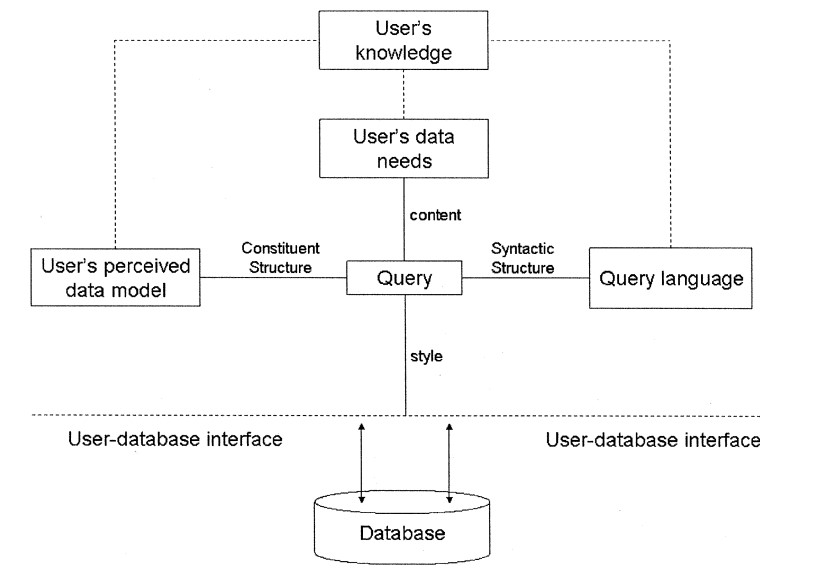
\includegraphics[width=\linewidth]{figures/cognitive_mapping_techniques_for_user_database_interaction_fig_1.jpg}
%   \caption{Sequential Framework for user-database interaction \cite{1637793}}
%   \label{fig:sequential_framework}
% \end{figure}

During this sequential query formulation process, users must contend with human factors-based challenges including cognitive strain, heuristic-driven biases, satisficing, and automaticity, all of which may negatively impact query accuracy and a user's ability to meet their data needs~\cite{1637793}. 
In cases where a query fails to fulfill a user's data needs, an answer understanding and response process may help users make corrections to a faulty query and to steer the query toward their original query intent.

The automatic interactive data exploration framework (depicted in figure \ref{fig:interactive_framework}) addresses user data needs that contain higher levels of uncertainty. This is done through a process of interactive data exploration. 
\cite{10.1145/2588555.2610523} This interactive framework introduces a cyclical process of sample extraction and data exploration that aides users in refining queries prior to final execution. 
It may benefit users who are less familiar with database schema and content, and who must interact iteratively with a database in order to discover new insights or better understand their data needs.

\begin{figure}
  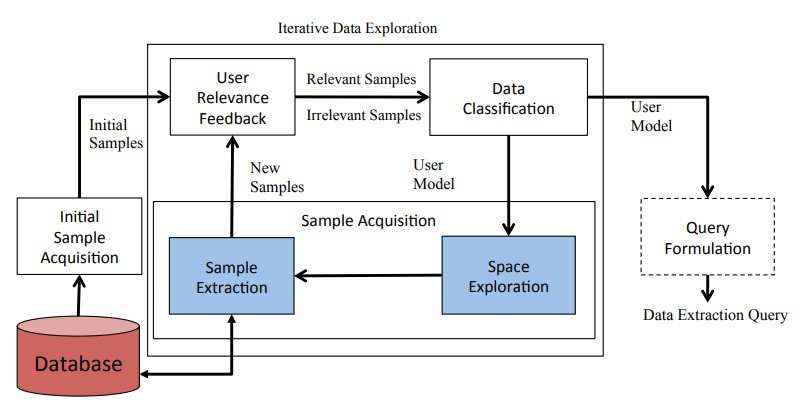
\includegraphics[width=\linewidth]{figures/explore_by_example_figure_1.jpg}
  \caption{Interactive Exploration Framework for user-database interaction \cite{10.1145/2588555.2610523}}
  \label{fig:interactive_framework}
\end{figure}

Similar to the interactive exploration framework, the stepwise approach \cite{10.5555/647248.719775} provides a simplified view of iterative query formulation and modification:

\begin{enumerate}
  \item Understanding - evaluate the schema in the context of a data need and develop a query subschema.
  \item Query formulation - express query operands involved in the intended query using the query subschema developed in the previous step.
  \item Testing - verify that the query expression formed in the prior step fulfills the user's data need.
\end{enumerate}

Interactive frameworks are enabled by the implementation of graphics-based direct manipulation interfaces, conversations with databases using natural language, optimized data sampling and interim result presentation, and other combinations of both familiar and novel techniques.

\subsection{Levels of Interaction}

There are three different levels of database interaction and data model abstraction: physical, logical and conceptual. Abstraction levels represent a transition of power and responsibility between database systems and their users. A high level of abstraction requires users to know less about the underlying physical data configuration and places responsibility on the system to know more about the model as it relates to the world, whereas a lack of abstraction requires users to understand the relationship between the world the data represents and the physical configuration of the data. \cite{10.2307/249587, 1268162} Humans generally interact with databases at the logical and conceptual levels, leaving the database management system to handle the physical-level implementation details.

\subsubsection{Conceptual} The highest level of abstraction, the conceptual level provides an ontological layer that represents real-world entities in domain-focused terms. 
Database users interacting at the conceptual level should not have to be concerned with the underlying data schema, logical contraints, and relationships between schema objects.

\subsubsection{Logical} The logical level serves as a linkage between the conceptual and physical levels. The database schema, including table and column names, views, and constraints, generally correspond with the logical level design of a database. Where possible, entities in a logical schema should remain recognizable as representations of real world objects. Languages such as SQL enable users to interact with databases at the logical level by expressing relational operations using a declarative syntax to extract data from a database.

\subsubsection{Physical} The introduction of declarative querying by using SQL has largely eliminated the need for users to interact with databases at the physical level. We now leave this task to the underlying database management system (DBMS). 
At this level, the DBMS employs its understanding of the schema definition, database constraints, indexing, file system, etc. to fulfill a human user's query intent by interpreting, optimizing, and executing their conceptual- or logical-level queries on the database system's file management and storage subsystem.


\subsection{Types of Interaction Interfaces}

There are multiple categories of database interaction methods including textual (linear keyword or computer language), visual (graphical), and natural language \cite{1637793}. These interfaces generally support a user's interaction with databases during the query formulation, translation, and writing stages. 

\subsubsection{Formal Language}

The most prolific formal database interaction language, and arguably the de-facto industry standard for relational data interaction, is the structured query language (SQL). 
SQL is a relationally complete and declarative language designed to enable interaction with relational data stores at the logical level. 
It was originally designed to improve database accessibility for non-programmers by abstracting away the procedural instructions required to retrieve data from a data store. 
It replaces this process with a declarative language based on relational calculus and relational algebra~\cite{Chamberlin1974}. 
While SQL succeeded in this regard, aspects of its declarative syntax can still present a barrier to entry for those who wish to perform data retrieval and analysis tasks~\cite{10.1145/3514214, 10.1145/2729094.2742620}.

\subsubsection{Natural Language}

Natural language interfaces (NLIs) allow users to interact with databases using unstructured, or semi-structured, language. 
The NLI system takes on the responsibility of converting a user's natural language expression into a formal query that can be executed by the underlying database management system.

\subsubsection{Visual Querying}

Visual query systems employ graphical representations of database objects, relations and syntax-like operators to enable users to generate logical- or conceptual-level queries. 
One of the first such systems was Query by Example (QBE), which was a form-based visual system developed in the IBM Thomaas J. Watson Research Center in 1975 \cite{10.1145/1282480.1282482}. 
QBE, with its form-based format, makes use of skeleton tables which allow users to specify a query by entering an example of a possible answer into the tables. 
When compared to SQL, QBE has been found to reduce the amount of time to form a correct query as well as the number errors introduced during query creation \cite{223806}. Since the development of QBE, a myriad of visual query systems have been conceptualized and implemented.


\subsection{Technical Contributions}


\subsection{Practical Impact}


\subsection{Summary}